\label{sec:results}
 
We implemented the CSA-MDP algorithm using the XADD representation and tested it on several domains. Apart from the \MarsRoverNL, we considered problems from the OR
literature such as \InventoryControl and \WaterReservoir. In the following
section we study these examples empirically.
 
%%%%%%%%%%%%%%%%%%%%%%%%%%%%%%%%%%%%%%%%%%%%%%%%%%%%%%%%%%%%%%%%%%%%%%%%%%
%figure5 : time-iteration and space-iteraton for 1d-2d-noPrune inventory
\begin{figure*}[t]
\centering
%\subfigure{
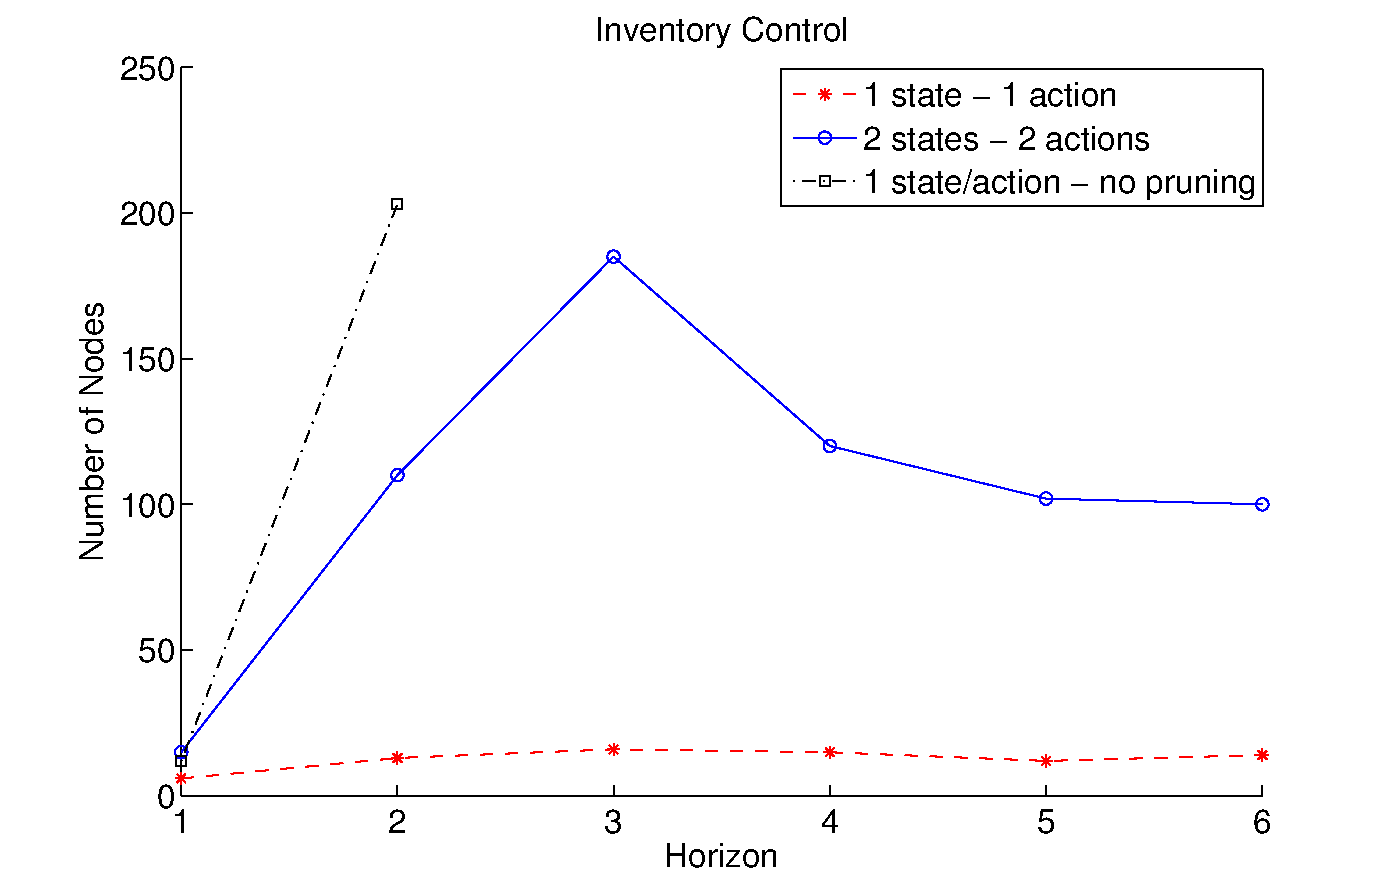
\includegraphics[width=0.47\textwidth]{Figures1/space1-3.pdf}
\hspace{5mm}
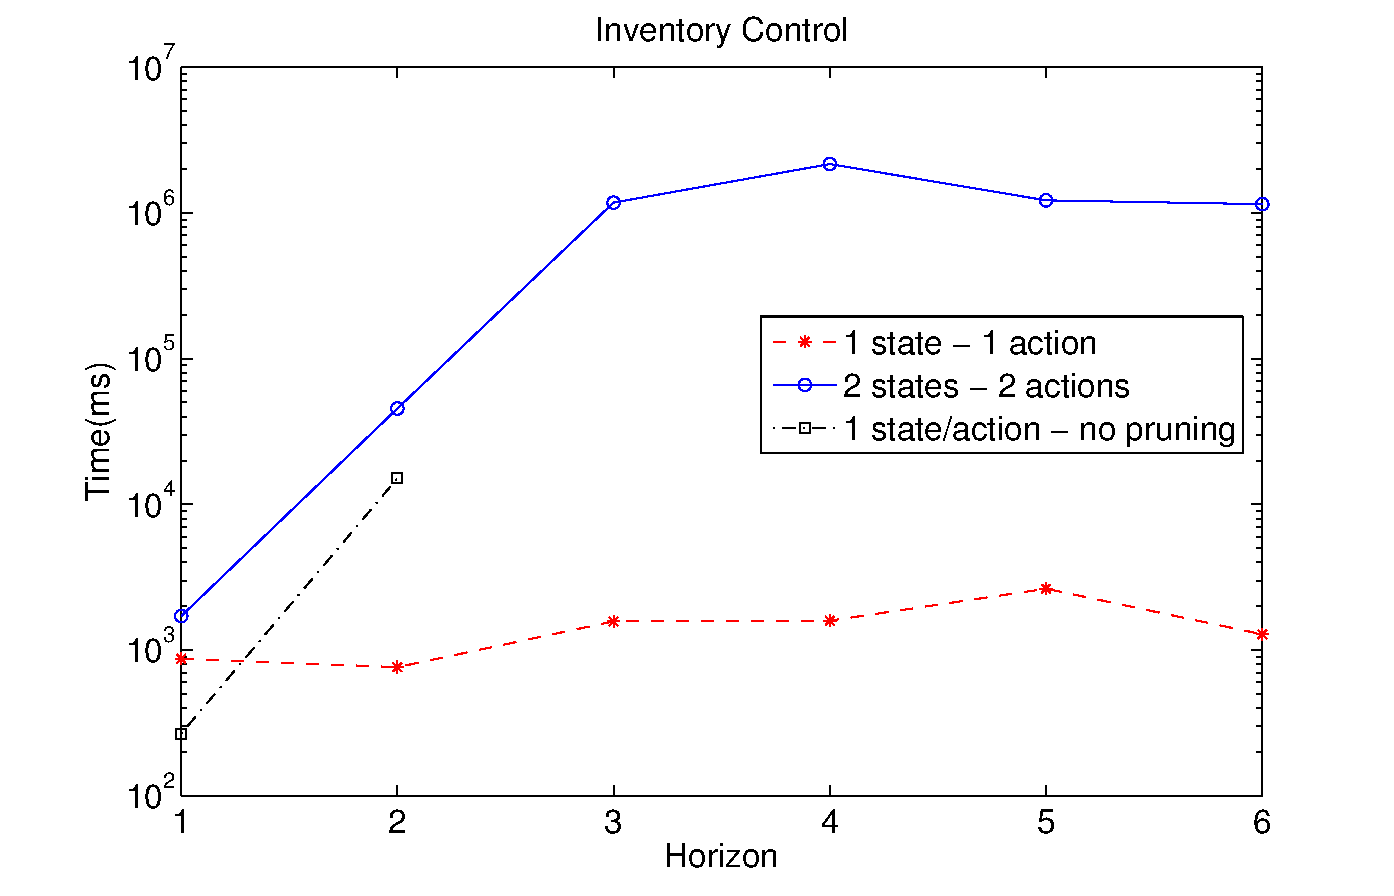
\includegraphics[width=0.47\textwidth]{Figures1/time1-3.pdf}
%}
%\vspace{-3mm}
\caption{\footnotesize
Space (\# XADD nodes in value function) and
time for different horizons of CSA-MDP on \InventoryControl\
Comparing 1D, 2D and no-pruning}
\label{fig:invC}
%\vspace{-3mm}
\end{figure*}
%%%%%%%%%%%%%%%%%%%%%%%%%%%%%%%%%%%%%%%%%%%%%%%%%%%%%%%%%%%%%%%%%%%%%%%%%%
 
\subsection{\InventoryControl}
This domain problem is a well-known optimization benchmark in the OR
literature. The inventory control theory is concerned with the decision problems of when to buy and how much to buy of a certain inventory item (inventory quantity or lot-size). The goal is to optimize a certain property of the system such as costs or profits. \cite{scarf_inv}

There are various costs related to any item in the inventory. Production/ procurement costs are used to benefit ordering large quantities in advance. Holding/storage costs are used as the trade-off against production costs as holding items in the inventory before the time required is expensive. Shortage/ penalty costs are considered when the inventory can not meet the customer requirements. Demand levels are another source for holding inventories in case future requirements change deterministically or in a stochastic manner. 
% we can take this part out:
We consider our model as a variation of Scarf's general inventory control model:
 
\paragraph*{Scarf's (S,s) policy:}
%single item, discrete time, deterministic demand, no capacity constraints
The (S,s) policy is a wide spread policy used in practise which considers a policy with the two constant s,S such that: 
\[y = \begin{cases}
S & if x<s \\
x & if x \geq s
\end{cases}\]

where y is the inventory level and x is the order quantity.  A deterministic model of the inventory theory is defined so that all cost prices and demands are known with certainty. 

The formal MDP definition of this problem is as below:
\begin{itemize}
\item y = State of the single-item inventory stock
\item x = Action for ordering (quantity to order) 
\item Transition function $y = y + x - \varphi(t) $ where $\varphi$ is the density of the demand distribution.
\item Reward function $R = -C(x) = c(y-x)+L(y)$ which is the negative expected cost function with c(z) as the ordering cost and L(y) as the expected holding and shortage costs defined below: 
\[ 
L(y) =\int_0^y \! h(y-\xi)\varphi(\xi) \, \mathrm{d} xi + \int_y^{\infty} \! p(\xi - y)\varphi(\xi) \, \mathrm{d} \xi 
\]
where p() is the shortage cost function, h() the holding cost function and $\varphi$ the density of the demand distribution. 
\end{itemize}

% end of scarf's policy

We present a simple formulation of this problem with a maximum capacity C for the inventory. This capacitated version is proved to be an NP-hard problem \cite{bitran} and more complicated than its uncapacitated counterparts. Assuming customer orders not satisfied in this month are backlogged for the next month, allows inventory to take negative values. 

We consider three capacitated problem instances, a one product inventory with one order action, a two product inventory that needs two different orders with stochastic demand and a three product, 3 orders with deterministic demand.
We present the mathematical formulation of the two product-two order case, the other two domains are modelled similarly. We take two continuous state variable $x_1,x_2$ indicating the current inventory quantity, with the total inventory capacity of 200, and a stochastic boolean state variable for customer demand level $d$ where $d=0$ is low demand levels (50) and $d=1$ is high demand levels (150) according to some probability. The continuous action variable is the order quantity $a_1,a_2$.The transition for one of the state variables is defined below:
 
{\footnotesize
\begin{align*}
x'_1 & = \begin{cases}
d \wedge (x_1 + a_1 + x_2 - 150 \leq 200) : & x_1 + a_1 - 150 \\
d \wedge (x_1 + a_1 + x_2 - 150 \geq 200) : & x_1 - 150 \\
\neg d \wedge (x_1 + a_1 + x_2 - 50 \leq 200): & x_1 + a_1 - 50 \\
\neg d \wedge (x_1 + a_1 + x_2 - 50 \geq 200): & x_1 - 50 \\
\end{cases}\\
\end{align*}}
% write description in case we have to take this huge case out!
The transition for the continuous actions partitions based on the maximum
capacity of the inventory (for both products), and only adds the orders if
the current total capacity (with respect to the orders of that product and
the stocks available for both products) are less than this maximum capacity.The demand variable is transitioned stochastically. 
{\footnotesize
\begin{align*}
d' & = \begin{cases}
d : &(0.7)\\
\neg d: &(0.3)\\
\end{cases}\\
\end{align*}}
Next we define an immediate negative reward for the cost of producing an order
and the storage cost of holding the products in the inventory and a
positive reward for fulfilling the customer demand whenever there are enough
stocks in the inventory. The total reward is the sum of the following two reward functions:
      			
{\footnotesize
\begin{align*}
R_1 & = \begin{cases}
(x_1 \geq 150) \wedge d :& 150 - 0.5\times a_1 - 0.1\times x_1 \\
\neg(x_1 \geq 150) \wedge d :& 150 - 0.5\times a_1 - 1.1\times x_1 \\
(x_1 \geq 50) \wedge \neg d :& 50 - 0.5\times a_1 - 0.1\times x_1 \\
\neg (x_1 \geq 150) \wedge \neg d :& 50 - 0.5\times a_1 - 1.1\times x_1 \\
\end{cases}
\end{align*}}
\\
+
\\
{\footnotesize
\begin{align*}
R_2 &= \begin{cases}
(x_2 \geq 150) \wedge d :& 150 - 0.4\times a_2 - 0.1\times x_2 \\
\neg(x_2 \geq 150) \wedge d :& 150 - 0.4\times a_2 - 0.1\times x_2 \\
(x_2 \geq 50) \wedge \neg d :& 50 - 0.4\times a_2 - 0.1\times x_2 \\
\neg (x_2 \geq 150) \wedge \neg d :& 50 - 0.4\times a_2 - 0.1\times x_2 \\
\end{cases}
\end{align*}}
 
The reward function is based on demand levels and current stock in inventory. If the current stock is larger than the total inventory, we get rewarded for
fulfilling the demand $(e.g 150)$, if the demand is high or if the inventory
is not high enough, then the reward is $(e.g (150 - (x_1+x_2)))$, in both
cases action order costs are added. This allows the
inventory to stock as many products as possible while not exceeding the
capacity of the inventory.
 
We plot the results of comparing different \InventoryControl problem sizes: 1-State,1-Action with stochastic demand (1SA,SD), 2-State,2-Action with stochastic and deterministic demand (2SA,SD ; 2SA,DD) and a 3-State, 3-Action with deterministic demand (3SA,DD). Figure~\ref{fig:invC} compares the time and space
for different iterations for these problems instances and an extra
comparison for the effect of not pruning on the 1D instance. 

Comparing different problem sizes demonstrates the effect of the number of action variables in our algorithm. As the problem size increases, both action and states effect the time and space required to perform the algorithm. CSA-MDP claims exact results for these problem instances therefore it iterates on all possible state-action partitions to find the optimal policy. 

The time and space have increased from the first iteration up to the third
iteration for the 2D problem size, but then dropped for the next horizons
due to pruning the XADD in our algorithm. As more constraints got added in
for horizon 4, they cancelled the effects of some of the previous branches
because of infeasibility and the pruning operation allows the XADD to grow
smaller in space and requiring almost a constant time depending on the
constraints added in each horizon.

For the 2-state-action problem, we considered two variations with constraints such as holding costs or total inventory capacity. Results show that adding holding costs to the problem does effect the complexity of the problem. In general adding state or action variables in the reward function can increase the XADD size. The holding cost adds the following constraint to all branches in the reward function: 
$ -0.1*x1 -0.1*x2 $
In another simulation, we tested adding all the products to the inventory constraints such that the transition function is conditioned on both products and their future orders:  $x'_1 = (x_1 + a_1 + x_2 +a_2 - 150 \leq 200) $. This version requires more space since replacing each of the action variables with their related bounds adds to the decision nodes.
Stochastic demands force more partitions for a problem instance as the plots for the 2-state-action case shows. Although the result for 1d stochastic is impressive, but for the 2d case, stochastic demand forces complexity. This partitioning occurs in the Q-function where the final result considers the restriction to the stochastic variable values. 

Without considering pruning, even the 1 product problem instance quickly falls into the curse of dimensionality problem. In fact, after the second iteration time and space grows exponentially and for this reason the plot fails to show the next time and
space.


%%%%%%%%%%%%%%%%%%%%%%%%%%%%%%%%%%%%%%%%%%%%%%%%%%%%%%%%%%%%%%%%%%%%%%%%%%%
%% v2plot.pdf, Q-drain, Q-noDrain.pdf
%% annotation?
%\begin{figure*}[t]
%\centering
%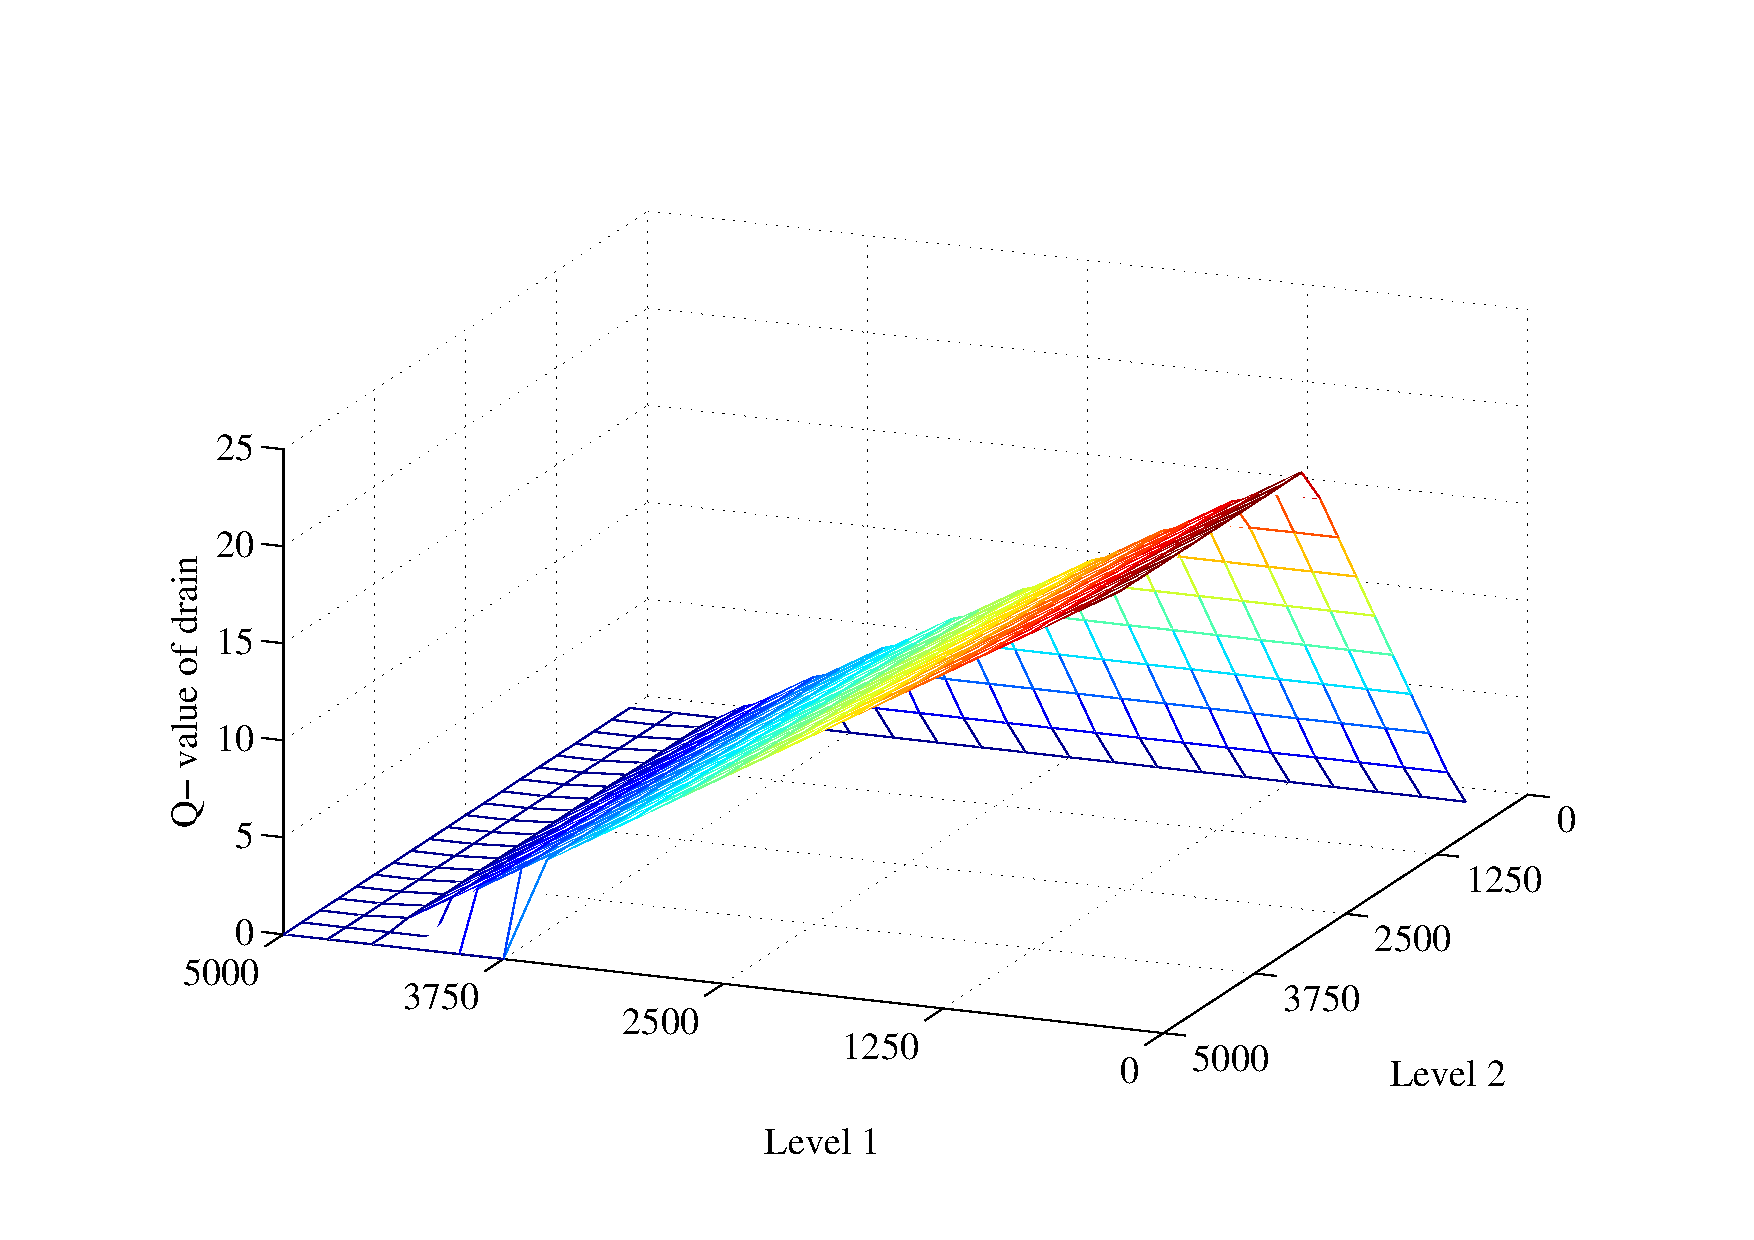
\includegraphics[width=0.33\textwidth]{Figures1/reservoir/Q2-Drain.pdf}
%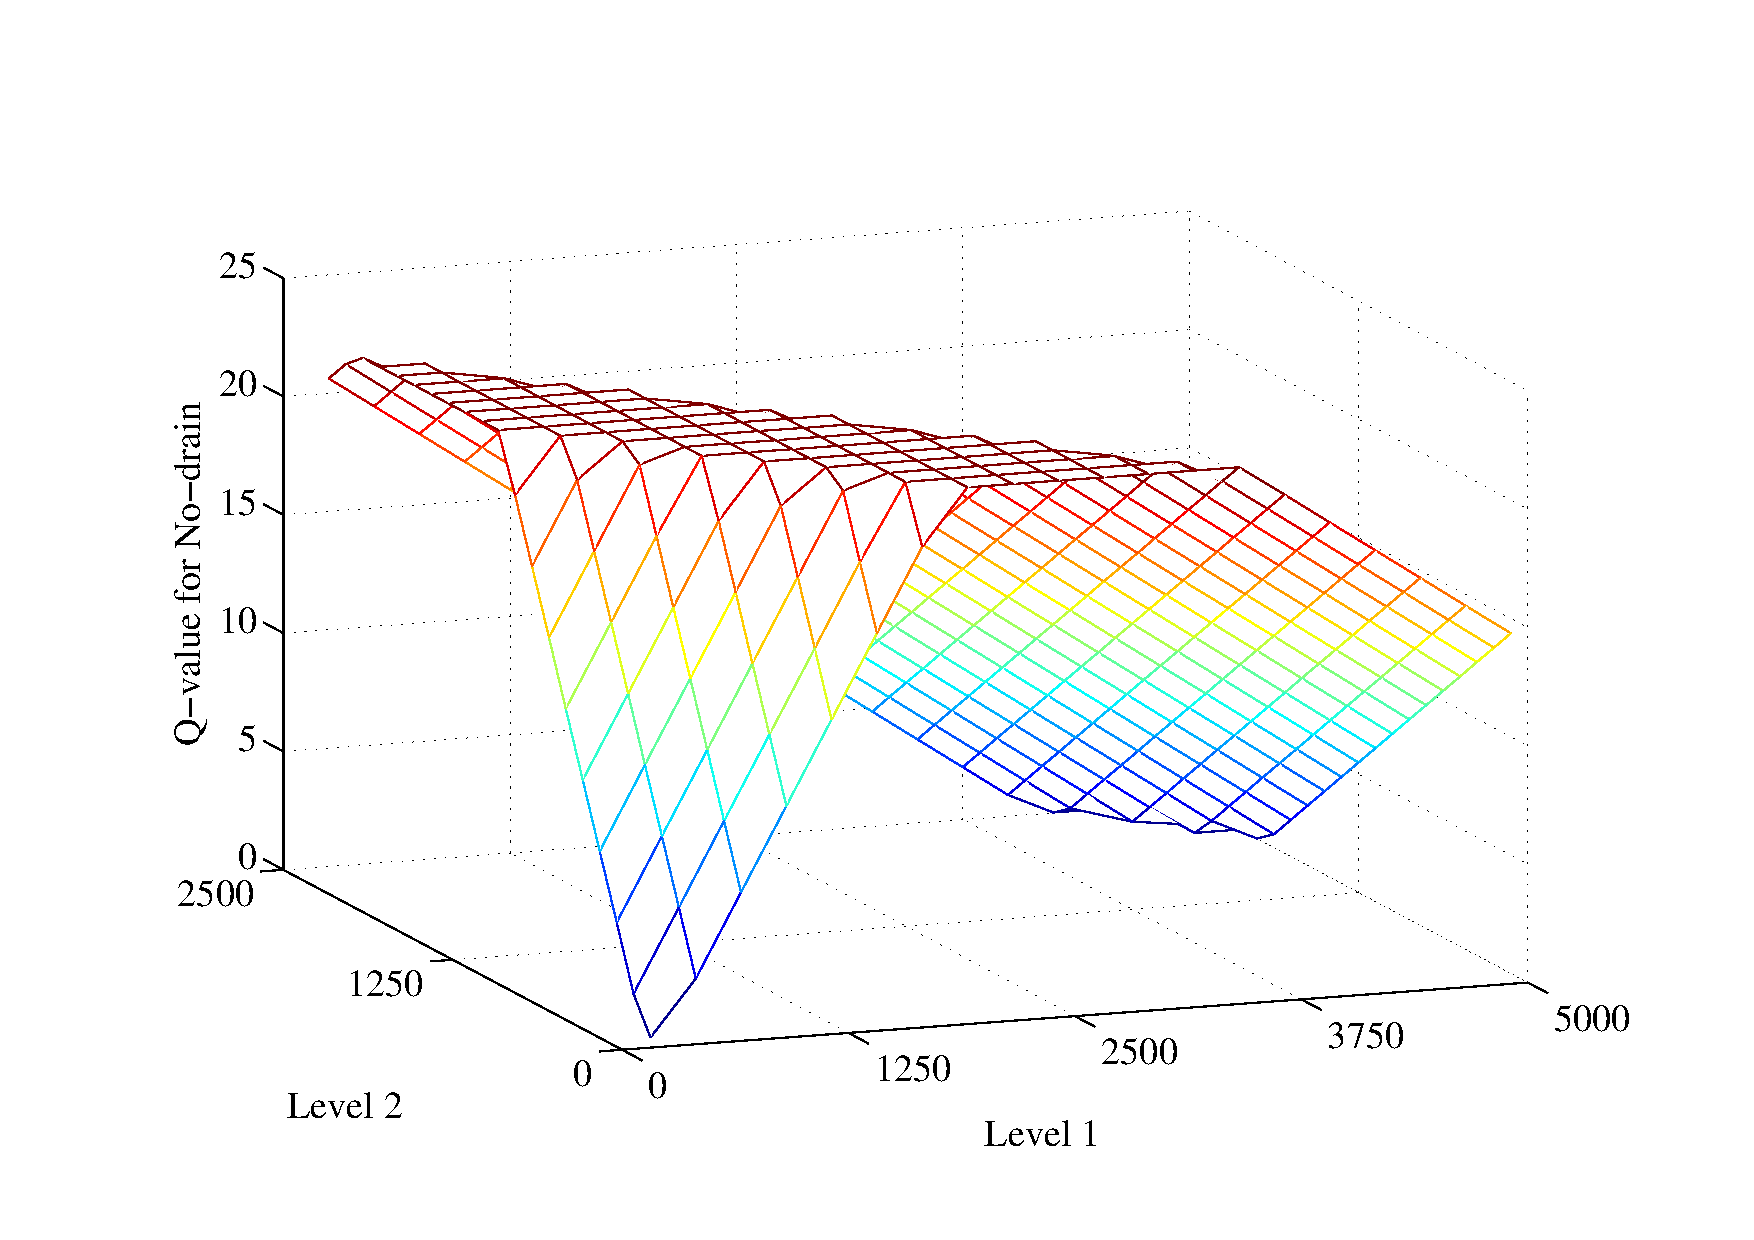
\includegraphics[width=0.33\textwidth]{Figures1/reservoir/Q2-noDrain.pdf}
%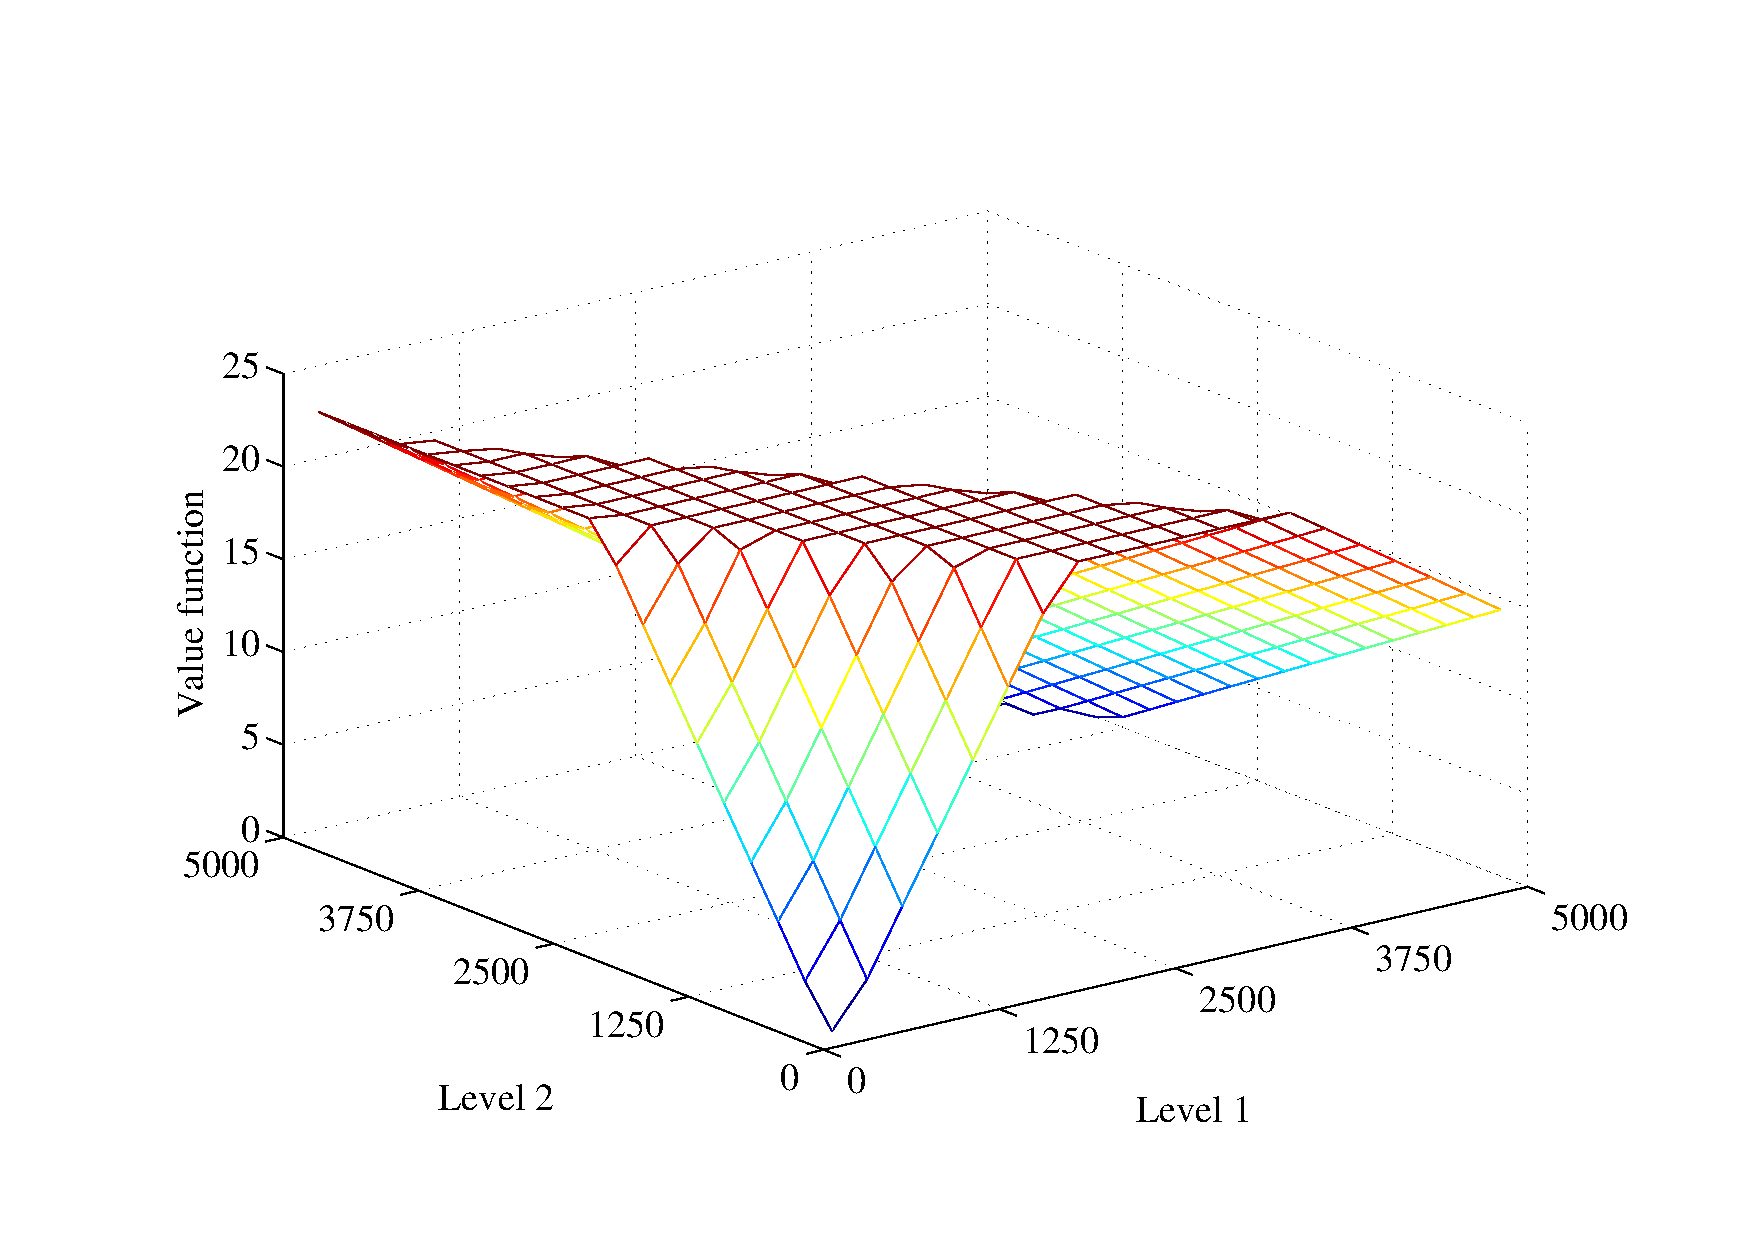
\includegraphics[width=0.33\textwidth]{Figures1/reservoir/v2plot.pdf}
%\caption{%\footnotesize 
%Value function and Q-function values of actions: Drain, No-Drain for second iteration
%}
%\label{fig:v2plots}
%%\vspace{-3mm}
%\end{figure*}
%%%%%%%%%%%%%%%%%%%%%%%%%%%%%%%%%%%%%%%%%%%%%%%%%%%%%%%%%%%%%%%%%%%%%%%%%%% 
% %%%%%%%%%%%%%%%%%%%%%%%%%%%%%%%%%%%%%%%%%%%%%%%%%%%%%%%%%%%%%%%%%%%%%%%%%%
%% v9plot.pdf, Q-drain, Q-noDrain.pdf
%\begin{figure*}[t]
%\centering
%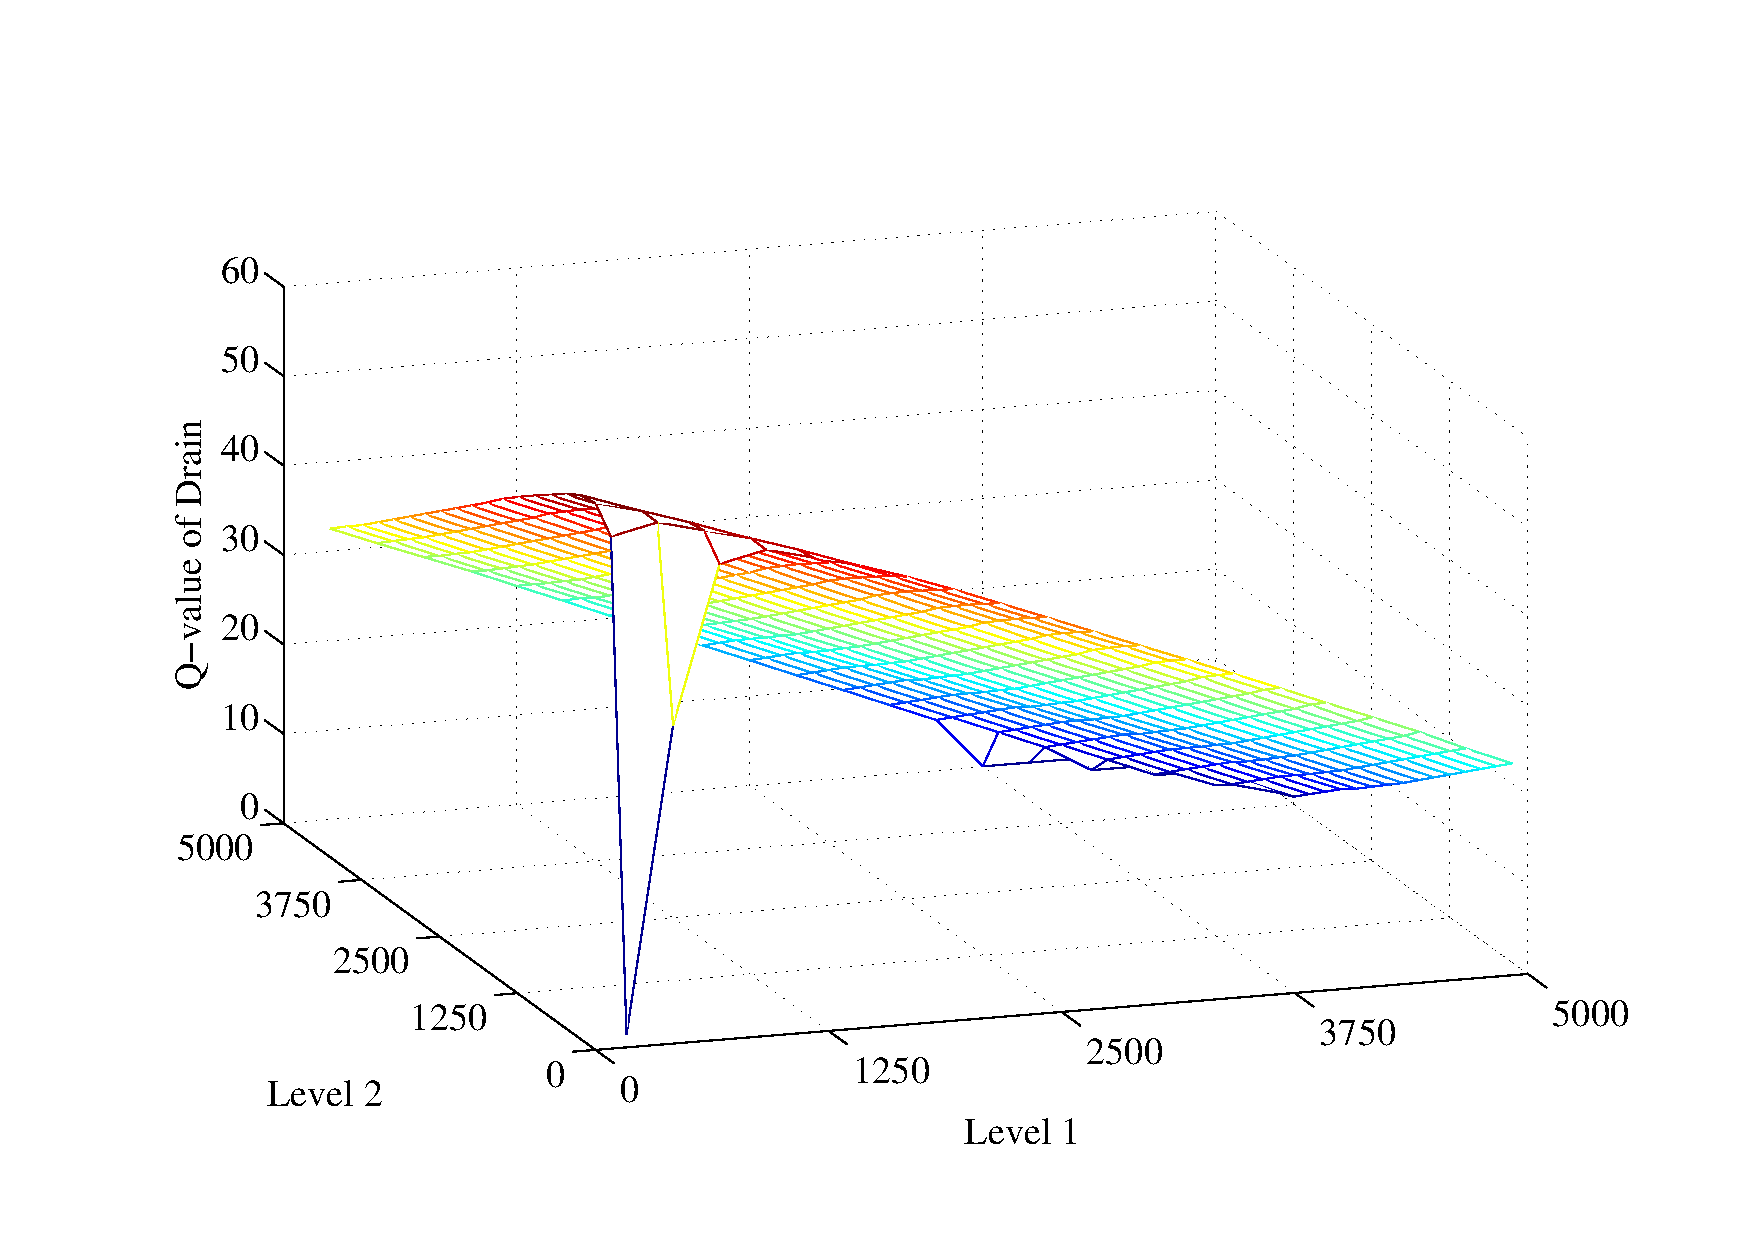
\includegraphics[width=0.33\textwidth]{Figures1/reservoir/Q9-Drain.pdf}
%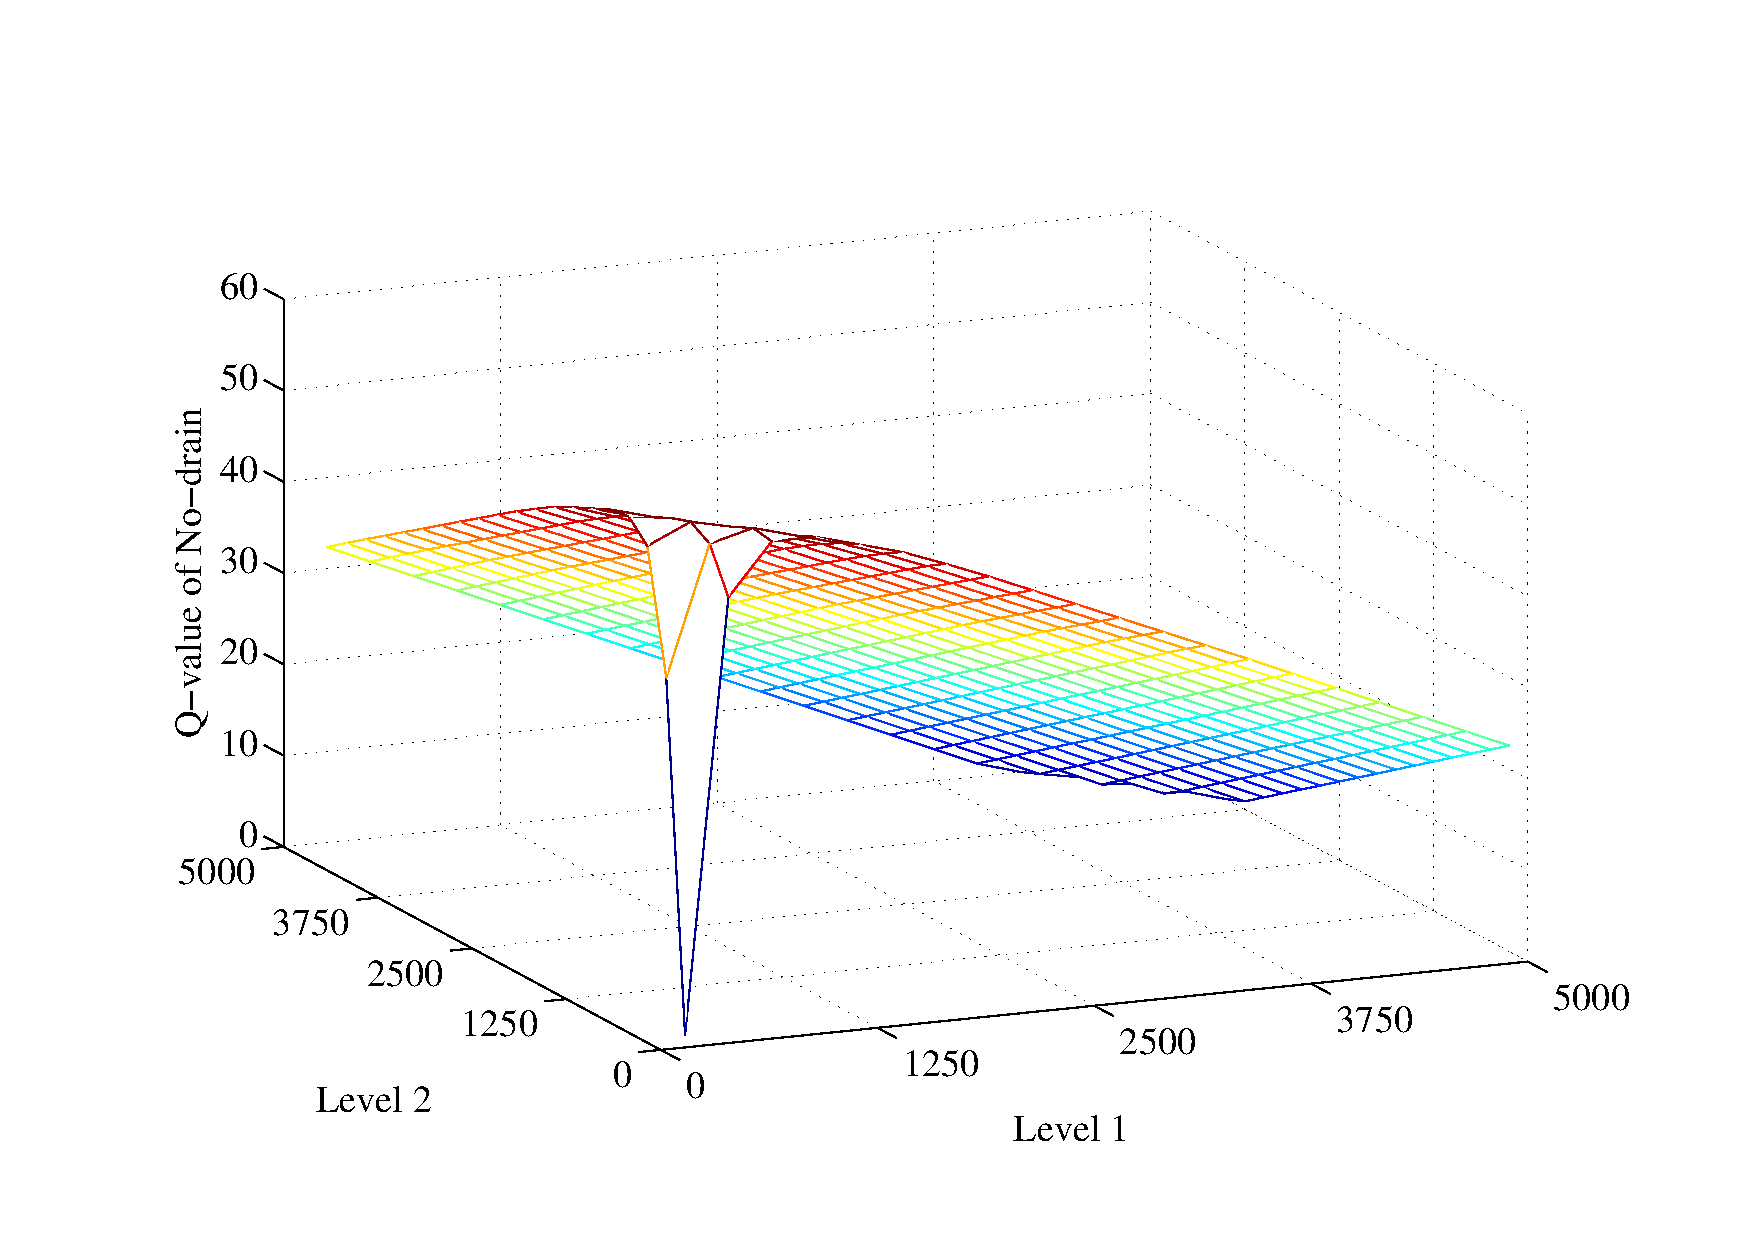
\includegraphics[width=0.33\textwidth]{Figures1/reservoir/Q9-noDrain.pdf}
%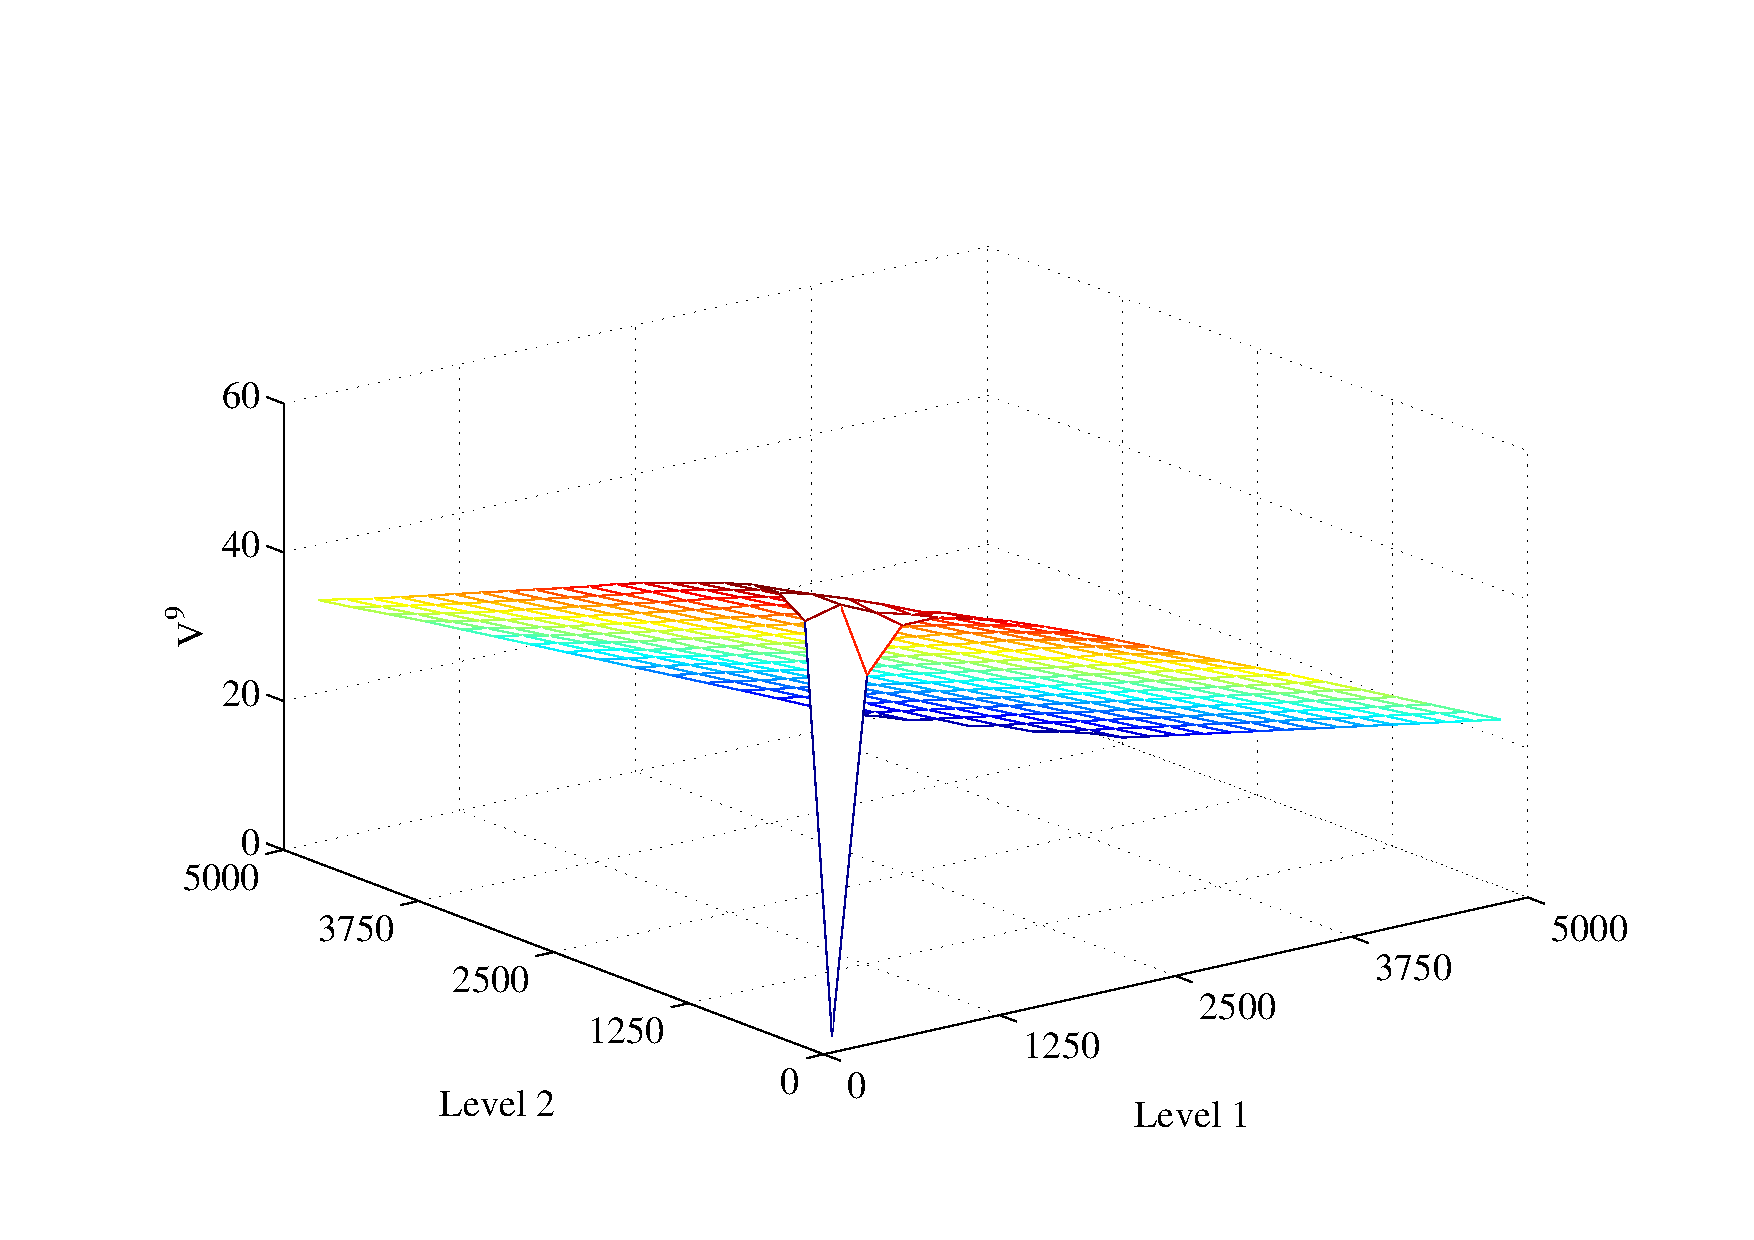
\includegraphics[width=0.33\textwidth]{Figures1/reservoir/v9plot.pdf}
%\caption{%\footnotesize 
%Value function and Q-function values of actions: Drain, No-Drain for the 9th iteration
%}
%\label{fig:v9plots}
%%\vspace{-3mm}
%\end{figure*}
%%%%%%%%%%%%%%%%%%%%%%%%%%%%%%%%%%%%%%%%%%%%%%%%%%%%%%%%%%%%%%%%%%%%%%%%%%% 

 %%%%%%%%%%%%%%%%%%%%%%%%%%%%%%%%%%%%%%%%%%%%%%%%%%%%%%%%%%%%%%%%%%%%%%%%%%
%policy
\begin{figure*}[t]
\centering
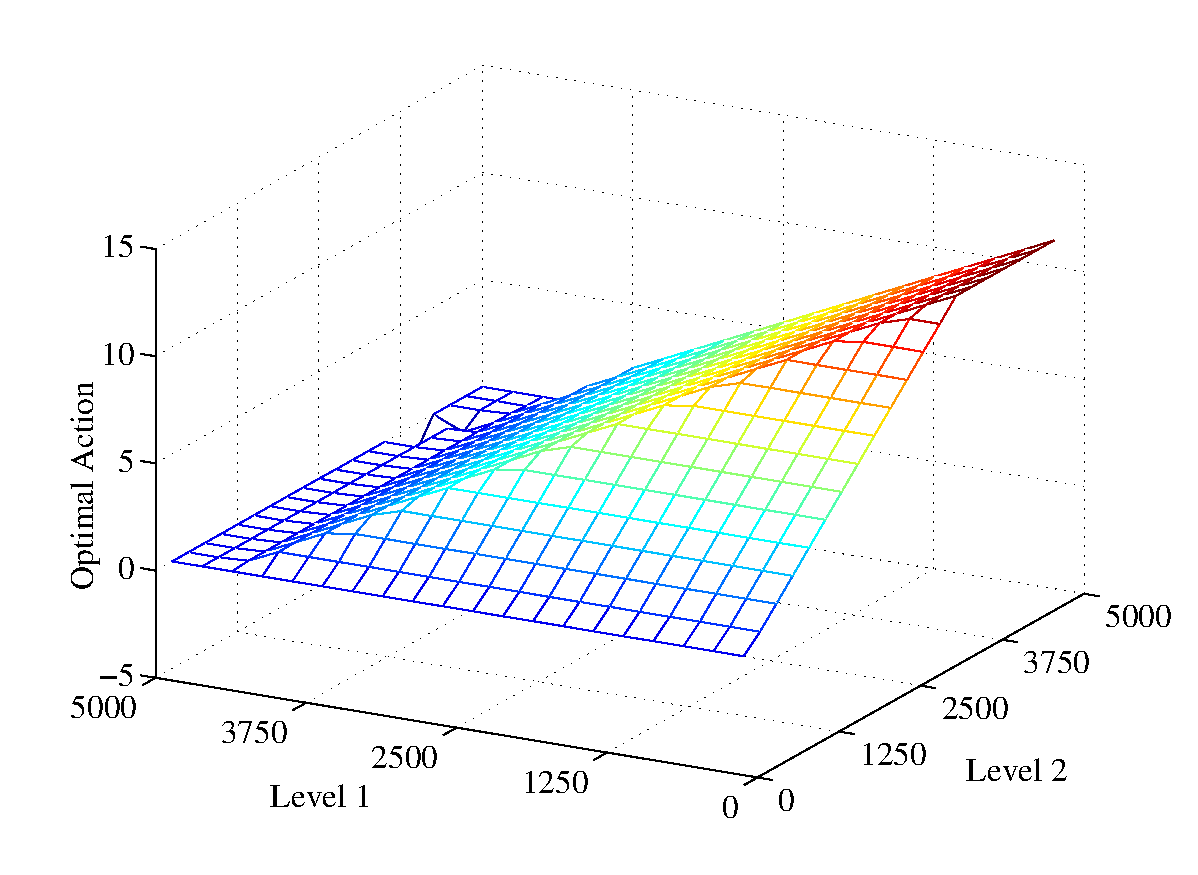
\includegraphics[width=0.47\textwidth]{Figures1/reservoir/policy-iteration2.pdf}
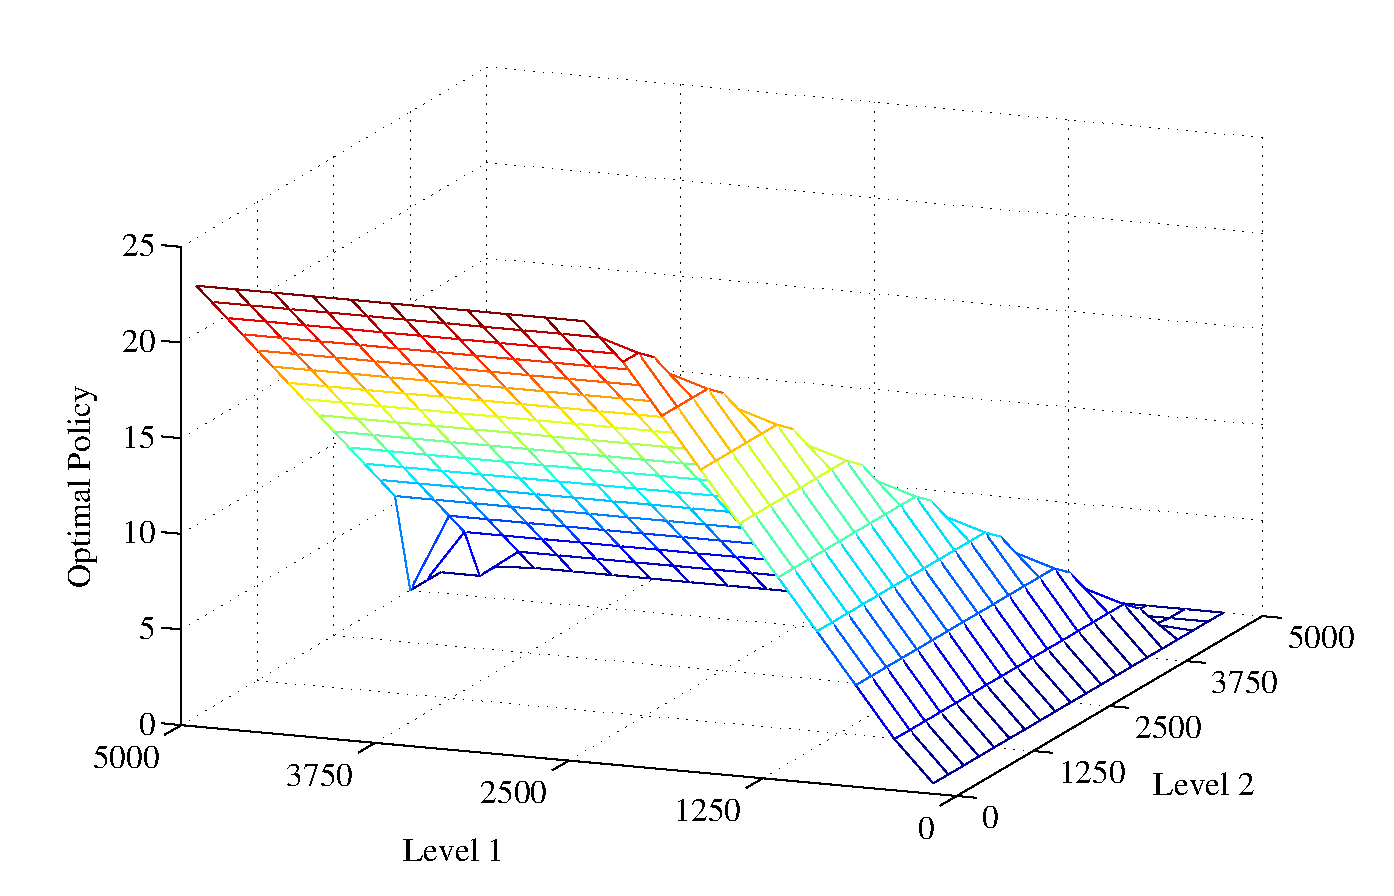
\includegraphics[width=0.47\textwidth]{Figures1/reservoir/policy-iteration3.pdf}
\caption{%\footnotesize 
Optimal policy for iteration 2 and 3
}
\label{fig:policyplots}
%\vspace{-3mm}
\end{figure*}
%%%%%%%%%%%%%%%%%%%%%%%%%%%%%%%%%%%%%%%%%%%%%%%%%%%%%%%%%%%%%%%%%%%%%%%%%% 
\subsection{\WaterReservoir}

In this experiment, we consider a continuous-time approach for the multi-reservoir domain.  
The problem of \WaterReservoir  needs to make an optimal decision on how much and when to discharge water from water reservoirs to maximize hydroelectric energy productions while considering environment constraints such as irrigation requirements and flood prevention. 

A multi-reservoir system is more desirable than the single reservoir problem due to its ability in controlling various environment parameters such as flooding.  In these systems, the inflow of downstream reservoirs are affected by the outflow of their upstream reservoirs. In the OR literature, this case  is considered much more complex and for the sake of simplicity mainly the single case in considered. For multi-reservoirs the main problem that leads to approximations to DP methods or sampling approaches is the curse of dimensionality \cite{Mahootchi2009}. Our approach handles this complexity using continuous states and actions.

The objective in this example is to find the optimal time for draining the reservoirs so that maximum reward is obtained. If draining occurs too frequently (in small time frames), flooding may occur from the excess water. This means draining should occur as latest as possible. On the other hand, not draining will cause overflow of the reservoir and waste of the energy. 

The MDP solution should solve a policy that obtains the maximum profit of electricity charges, while staying in the safe water levels of both reservoirs. In order to consider the time as a continuous variable, we allowing the system to choose to drain at any time. The choice of not draining will not gain any profit as we reward according to the electricity discharged. Two discrete actions of drain and no-drain is considered where the former is a of a continuous-time  nature. The transition function is demonstrated below: 

{\footnotesize
\begin{align*}
x_1'  = 400 * e + x1 -700 * e + 500 * e \\
x_2'  = 400 * e + x2 - 500 * e \\
\end{align*}
}
Here we take draining as the act of discharging water levels per time-step from the upper-stream reservoir to the down-stream reservoir ($500 * e$). A constant amount of discharge is always considered for the down-stream to ensure all electricity demands are fulfilled.  The amount of rain (r) is considered as a constant(400)which affects both reservoirs at the time of discharge. 

The reward function for both actions considers the safe range of [50,4500] as the safe water levels and assigns a positive reward of $e$ for the action of draining, and no rewards ( but also no penalty) for not draining. If the next state is not in the safe range, a huge penalty of -1+e6 is assigned as the reward:

{\footnotesize
\begin{align*}
(x_1\leq 4500 - 200 * e) \wedge (x2 \leq 4500 +100 *e) \\
\wedge (x_1\geq 50 - 200 * e) \wedge (x2 \geq 50 +100 *e) : e \\
\end{align*}
}
We have presented the results for this experiment next. Because of the two actions and the fact that one is continuous, we would expect to see a draining action in one iteration and a no-drain action in the next iteration, since two  draining could be performed in one longer step.

The first iteration starts with a drain only policy and achieves the value according to the current water levels of both reservoirs. The up-stream reservoir obtains the maximum value function if it has water levels above half of the safe range. The value decreases as water levels in the down-stream reservoir goes higher due to flood prevention. 

We have demonstrated the optimal policy for the next two consequent iterations. In the second iteration, CSA-MDP will not drain the water because of the continuous nature of the problem, the required draining was performed in the previous iteration. As the water levels increase, 


 
%In figure \ref{fig:v2plots}, both Q-values of drain and no-drain for the second iteration have been visualized. As expected the value function follows from selecting the no-drain action. The Q-value of draining is similar to that of the first iteration and the final value function is similar to the Q-function of no-drain. The difference of the recent two value functions is in the fact that since draining was performed in the first iteration, in the second iteration, the down-stream reservoir is not in danger of flooding and can obtain the optimal value (22.5). Since flooding is a direct result of excess water in $x_1$, the optimal value is for the lower range levels in the down-stream compared to the levels of $x_2$. 
%
%
%Further iterations of the exact CSA-DP algorithm results in more partitions on the state-action space. The optimal policy converges to the value obtained in the second iteration. There are some minor difference in the value of each iteration due to the fact that with higher horizons, the reservoir can plan to obtain higher rewards and prevent flooding or overflowing. We provide the Q-values of draining, not draining and the value function for iteration 9 in \ref{fig:v9plots} to show this effect. 
%
%Also from this plot we want to confirm the fact that in the $9^th$ iteration, the policy should choose to drain (as all other odd-iterations). The difference between the Q-values of the two actions is very minor. The sum of distances between the value function and the two Q-values shows that this distance is 49.4887 for the drain action while it is equal to 90.5312 for the no-drain action. This shows that despite the small difference, the policy tends more towards draining in this iteration. 
